% =============================================================================
% PÓSTER CIENTÍFICO PROFESIONAL — 1 SOLA PÁGINA GARANTIZADA (A0: 841 x 1189 mm)
% Motor: tcolorbox [poster] (grilla exacta 6 columnas x 24 filas = 1 página)
% Compilar en Overleaf con pdfLaTeX
% =============================================================================
\documentclass[final]{article}

\usepackage[utf8]{inputenc}
\usepackage[T1]{fontenc}
\usepackage[a0paper, margin=0pt]{geometry}
\usepackage{lmodern}
\usepackage{anyfontsize}
\usepackage{graphicx}
\usepackage{xcolor}
\usepackage{booktabs}
\usepackage{tabularx}
\usepackage{enumitem}
\usepackage{amsmath,amssymb}
\usepackage[most]{tcolorbox}
\tcbuselibrary{poster}
\usepackage{tikz}
\usetikzlibrary{arrows.meta,positioning}

\pagestyle{empty}

% Paleta sobria de congreso científico / Ciberseguridad e Ingeniería
\definecolor{CINFBlue}{HTML}{122B4A}
\definecolor{CINFNavy}{HTML}{0F172A}
\definecolor{CINFRed}{HTML}{B4202A}
\definecolor{CINFAccent}{HTML}{0066CC}
\definecolor{CINFGreen}{HTML}{157A44}
\definecolor{CINFBg}{HTML}{E8EEF5}
\definecolor{CINFGray}{HTML}{475569}

\pagecolor{CINFBg}
\setlength{\parindent}{0pt}
\setlength{\parskip}{0.25cm}
\renewcommand{\familydefault}{\sfdefault}

\setlist[itemize]{leftmargin=1.1cm, itemsep=0.18cm, topsep=0.12cm}
\setlist[enumerate]{leftmargin=1.2cm, itemsep=0.18cm, topsep=0.12cm}

\begin{document}

% =============================================================================
% CONTENEDOR ÚNICO tcbposter: GARANTIZA EXACTAMENTE 1 PÁGINA SIN HUECOS
% Área útil A0: 80.1 cm ancho x 114.9 cm alto | Grilla: 6 cols x 24 filas
% =============================================================================
\noindent%
\begin{tcbposter}[
  coverage = {
    spread,
    left=1.8cm,
    right=1.8cm,
    top=1.8cm,
    bottom=1.8cm,
    interior style={fill=CINFBg},
    frame empty
  },
  poster = {
    showframe=false,
    columns=6,
    rows=24,
    spacing=7mm
  },
  boxes = {
    enhanced,
    colback=white,
    colframe=CINFBlue,
    coltitle=white,
    colbacktitle=CINFBlue,
    boxrule=2.2pt,
    arc=4.5mm,
    left=7mm,
    right=7mm,
    top=5.5mm,
    bottom=5.5mm,
    toptitle=3.5mm,
    bottomtitle=3.5mm,
    fonttitle=\bfseries\fontsize{22}{26}\selectfont\sffamily,
    fontupper=\fontsize{17.5}{22.5}\selectfont\sffamily,
    drop shadow={black!14}
  }
]

% -----------------------------------------------------------------------------
% FILAS 1-2: ENCABEZADO CIENTÍFICO PROFESIONAL
% -----------------------------------------------------------------------------
\posterbox[
  colback=CINFBlue,
  colframe=CINFNavy,
  boxrule=3pt,
  valign=center,
  left=11mm, right=11mm, top=4mm, bottom=4mm
]{name=header, column=1, span=6, row=1, rowspan=2}{%
  \begin{minipage}[c]{0.78\linewidth}
    {\color{white!78}\fontsize{19}{23}\selectfont\textbf{INVESTIGACIÓN TECNOLÓGICA APLICADA · CIBERSEGURIDAD E INTELIGENCIA ARTIFICIAL}}\\[3.5mm]
    {\color{white}\fontsize{39}{44}\selectfont\textbf{Sistema Centralizado de Detección de Anomalías en Redes IoT mediante Machine Learning}}\\[4mm]
    {\color{white!95}\fontsize{23}{27}\selectfont\textbf{Felipe Nicolás Vergara Rodríguez} \quad·\quad \textbf{Guía:} Nicolás Caselli Benavente \quad·\quad Facultad de Ingeniería, Universidad Andrés Bello}
  \end{minipage}\hfill
  \begin{minipage}[c]{0.19\linewidth}
    \centering
    \begin{tcolorbox}[colback=white, colframe=white, arc=3.5mm, left=3mm, right=3mm, top=3mm, bottom=3mm, halign=center, boxrule=0pt, no shadow]
      \IfFileExists{logo_ici.png}{%
        
\includegraphics[width=0.95\linewidth,height=4.8cm,keepaspectratio]{logo_ici.png}\\[2mm]
      }{}
      {\color{CINFBlue}\fontsize{15}{18}\selectfont\textbf{Ingeniería Civil Informática}}
    \end{tcolorbox}
  \end{minipage}%
}

% -----------------------------------------------------------------------------
% FILA 3: FRANJA DE 5 KPIs PRINCIPALES
% -----------------------------------------------------------------------------
\posterbox[
  colback=white,
  colframe=CINFNavy,
  boxrule=2pt,
  valign=center,
  left=5mm, right=5mm, top=2.5mm, bottom=2.5mm
]{name=kpis, column=1, span=6, row=3, rowspan=1}{%
  \centering
  \begin{minipage}[c]{0.19\linewidth}\centering
    {\fontsize{33}{36}\selectfont\bfseries\color{CINFBlue} 7,06 M}\\[1mm]
    {\fontsize{15}{18}\selectfont\color{CINFNavy}\textbf{Filas Auditadas}} {\fontsize{13}{16}\selectfont\color{CINFGray}(89 CSV · 0 NaN)}
  \end{minipage}\hfill
  \vrule width 1.5pt height 2.7cm\hfill
  \begin{minipage}[c]{0.19\linewidth}\centering
    {\fontsize{33}{36}\selectfont\bfseries\color{CINFGreen} 0,9995}\\[1mm]
    {\fontsize{15}{18}\selectfont\color{CINFNavy}\textbf{F1 Externo 6/2/1}} {\fontsize{13}{16}\selectfont\color{CINFGray}(FPR 0,14\% RF)}
  \end{minipage}\hfill
  \vrule width 1.5pt height 2.7cm\hfill
  \begin{minipage}[c]{0.19\linewidth}\centering
    {\fontsize{33}{36}\selectfont\bfseries\color{CINFRed} 39,90\%}\\[1mm]
    {\fontsize{15}{18}\selectfont\color{CINFNavy}\textbf{Recall Zero-Day}} {\fontsize{13}{16}\selectfont\color{CINFGray}(Sin Mirai, D4)}
  \end{minipage}\hfill
  \vrule width 1.5pt height 2.7cm\hfill
  \begin{minipage}[c]{0.19\linewidth}\centering
    {\fontsize{33}{36}\selectfont\bfseries\color{CINFAccent} 5,28 ms}\\[1mm]
    {\fontsize{15}{18}\selectfont\color{CINFNavy}\textbf{Latencia CPU}} {\fontsize{13}{16}\selectfont\color{CINFGray}(Meta $\le 10$ ms)}
  \end{minipage}\hfill
  \vrule width 1.5pt height 2.7cm\hfill
  \begin{minipage}[c]{0.19\linewidth}\centering
    {\fontsize{33}{36}\selectfont\bfseries\color{CINFNavy} 73 / 25}\\[1mm]
    {\fontsize{15}{18}\selectfont\color{CINFNavy}\textbf{Exp. / Tests OK}} {\fontsize{13}{16}\selectfont\color{CINFGray}(JWT · SHA-256)}
  \end{minipage}%
}

% -----------------------------------------------------------------------------
% FILAS 4-9 (ROWSPAN=6): FILA SUPERIOR DE 3 COLUMNAS
% -----------------------------------------------------------------------------
\posterbox[
  colframe=CINFBlue, colbacktitle=CINFBlue,
  title={1. Problema, Brecha y Defensa Perimetral}
]{name=box1, column=1, span=2, row=4, rowspan=6}{%
  Los dispositivos IoT domésticos (cámaras IP, timbres, termostatos) poseen CPU/RAM mínimas y firmware cerrado, impidiendo instalar agentes antivirus y facilitando su reclutamiento masivo por botnets (\textbf{Mirai} y \textbf{BASHLITE}).
  \begin{itemize}
    \item \textbf{Inspección centralizada:} Defensa perimetral en el Router/Gateway mediante metadatos de flujo (opera incluso sobre tráfico cifrado).
    \item \textbf{Brecha científica:} La literatura reporta $F1 > 99\%$ con \textit{splits} aleatorios o modelos por equipo (Meidan et al., 2018), ocultando fallas ante \textbf{hardware no visto} y \textbf{familias excluidas}.
  \end{itemize}
  \vfill
  \centering
  \IfFileExists{fig_ppt_topologia_iot.png}{%
    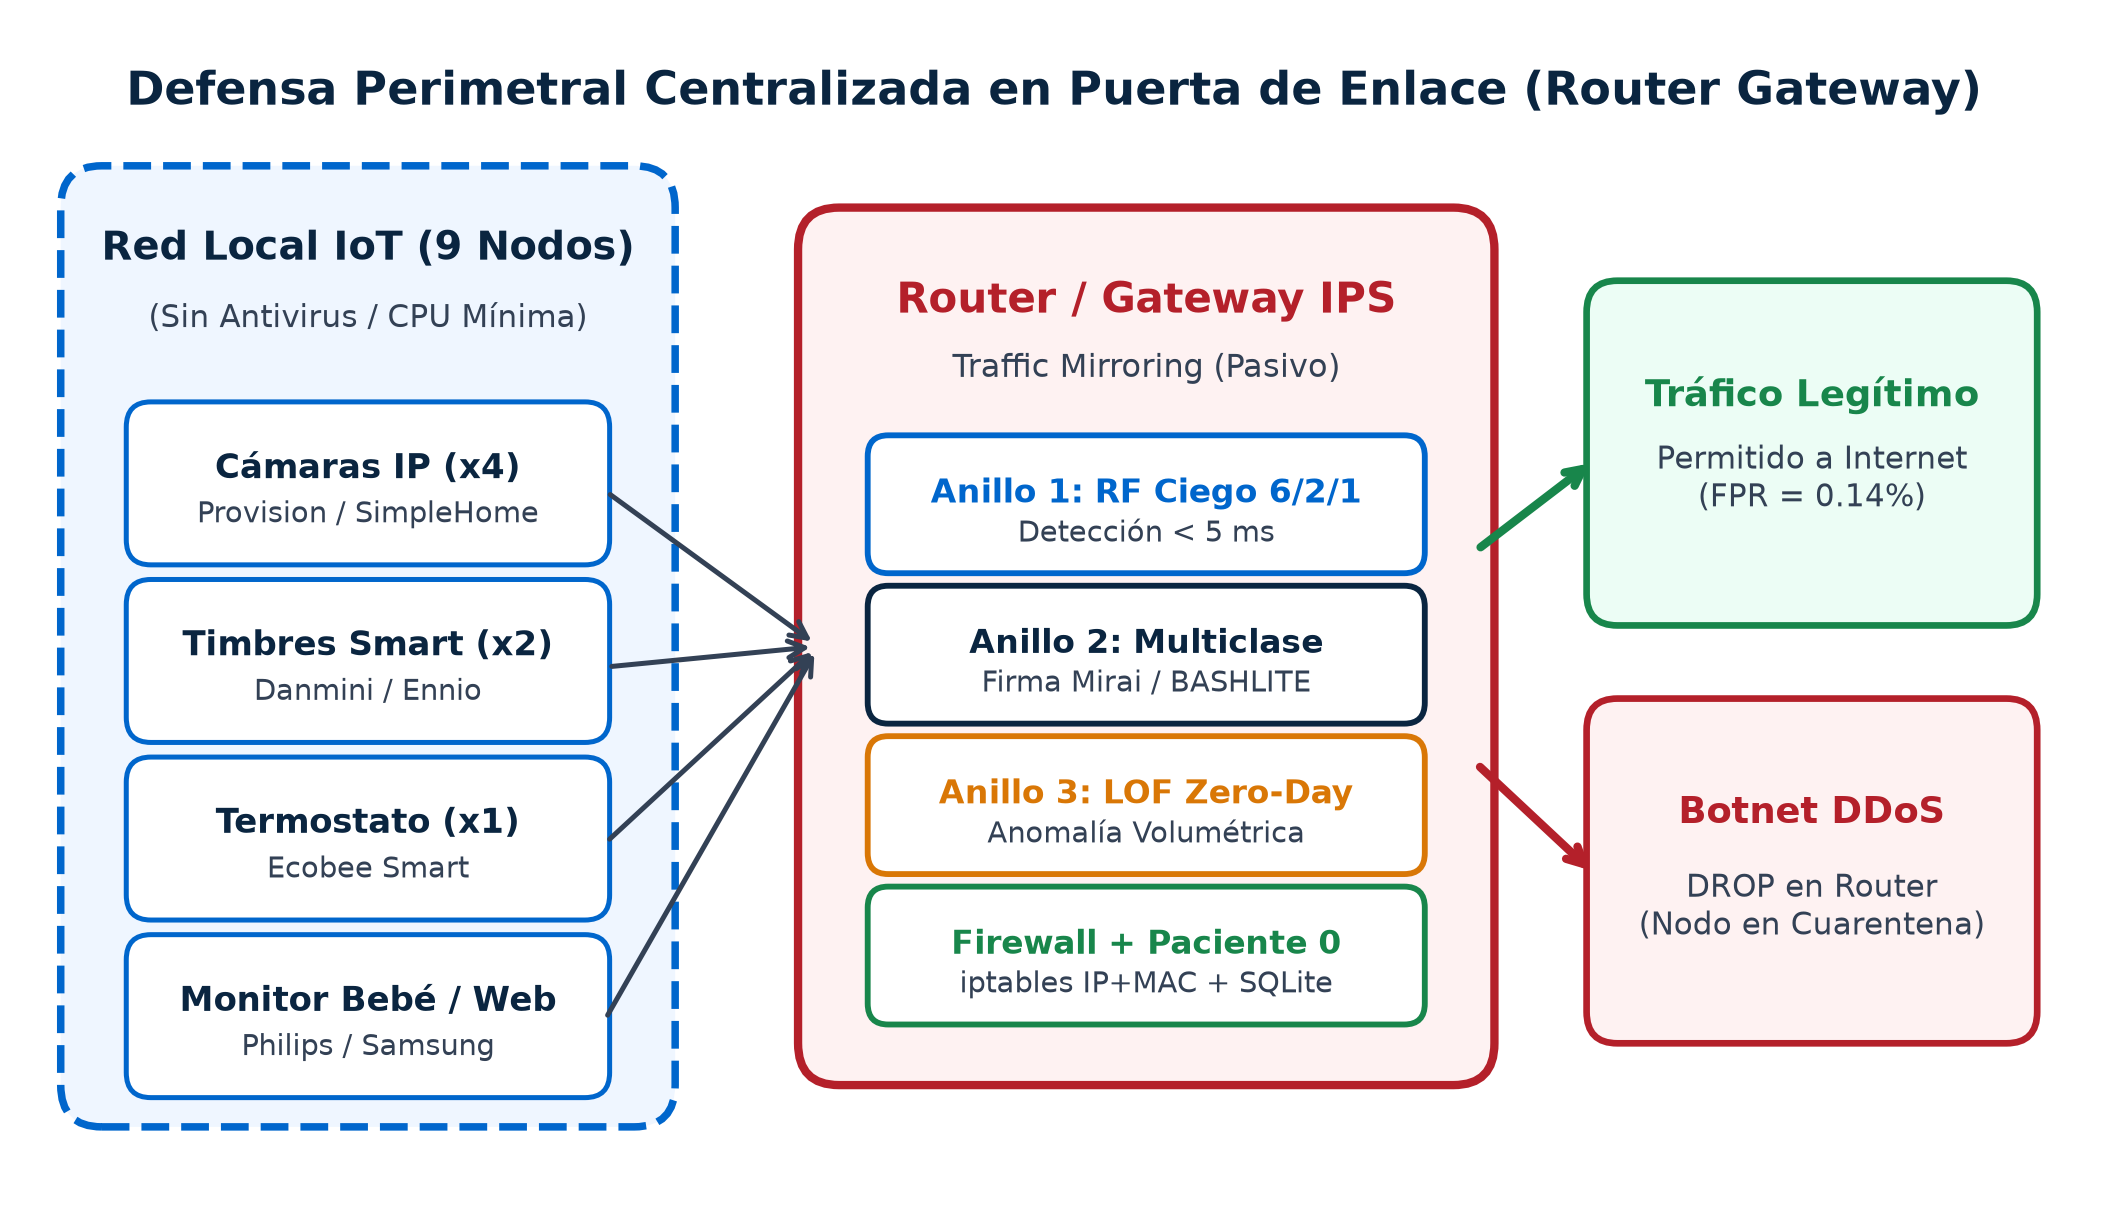
\includegraphics[width=0.98\linewidth,height=13.0cm,keepaspectratio]{fig_ppt_topologia_iot.png}\\[2mm]
  }{}
  {\fontsize{14}{18}\selectfont\color{CINFGray}\textbf{Figura 1.} Topología perimetral: 9 dispositivos IoT protegidos desde el Gateway con tres anillos de detección y mitigación.}
}

\posterbox[
  colframe=CINFNavy, colbacktitle=CINFNavy,
  title={2. Metodología Híbrida: CRISP-DM / CRISP-ML(Q) + Scrum}
]{name=box2, column=3, span=2, row=4, rowspan=6}{%
  Para articular ciencia de datos con desarrollo incremental de software se diseñó un marco de \textbf{doble capa}:
  \begin{itemize}
    \item \textbf{CRISP-DM + CRISP-ML(Q):} 6 fases iterativas reforzadas con \textbf{Aseguramiento de Calidad (Q)} contra fuga temporal, pruebas \textit{zero-day} e integridad \texttt{SHA-256}.
    \item \textbf{Scrum Adaptado:} Sprints 1--3 completados en 2026 y Sprints 4--7 proyectados para 2027, con \textit{Definition of Done} de 25 pruebas unitarias.
  \end{itemize}
  \vfill
  \centering
  \resizebox{0.99\linewidth}{!}{%
  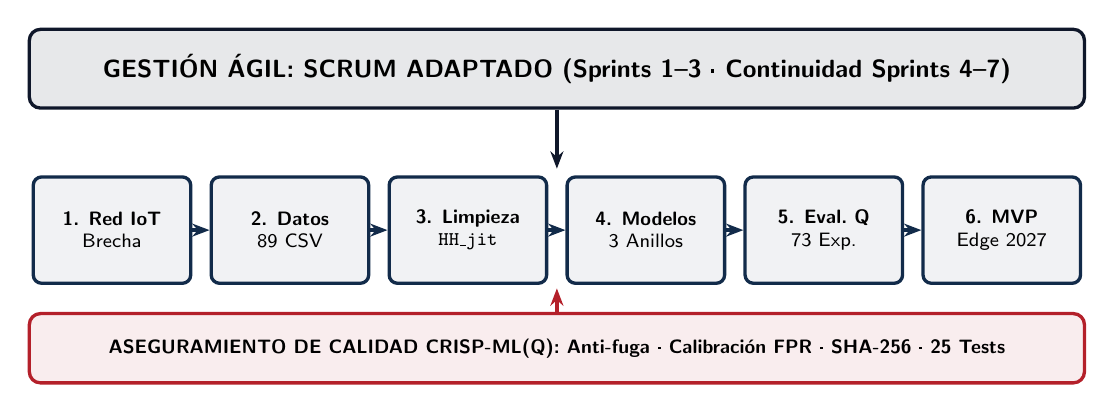
\begin{tikzpicture}[
    topb/.style={rectangle, draw=CINFNavy, fill=CINFNavy!10, very thick, rounded corners=4pt, minimum width=13.4cm, minimum height=1.0cm, align=center, font=\small\bfseries\sffamily},
    ph/.style={rectangle, draw=CINFBlue, fill=CINFBlue!6, very thick, rounded corners=3pt, minimum width=2.0cm, minimum height=1.35cm, align=center, font=\scriptsize\sffamily},
    qb/.style={rectangle, draw=CINFRed, fill=CINFRed!8, very thick, rounded corners=4pt, minimum width=13.4cm, minimum height=0.88cm, align=center, font=\scriptsize\bfseries\sffamily},
    arr/.style={-{Stealth[length=2.2mm]}, very thick, CINFBlue}
  ]
    \node[topb] (sc) at (0, 2.05) {GESTIÓN ÁGIL: SCRUM ADAPTADO (Sprints 1--3 · Continuidad Sprints 4--7)};
    \node[ph] (p1) at (-5.65, 0) {\textbf{1. Red IoT}\\Brecha};
    \node[ph] (p2) at (-3.39, 0) {\textbf{2. Datos}\\89 CSV};
    \node[ph] (p3) at (-1.13, 0) {\textbf{3. Limpieza}\\\texttt{HH\_jit}};
    \node[ph] (p4) at (1.13, 0) {\textbf{4. Modelos}\\3 Anillos};
    \node[ph] (p5) at (3.39, 0) {\textbf{5. Eval.\ Q}\\73 Exp.};
    \node[ph] (p6) at (5.65, 0) {\textbf{6. MVP}\\Edge 2027};
    \draw[arr] (p1)--(p2); \draw[arr] (p2)--(p3); \draw[arr] (p3)--(p4); \draw[arr] (p4)--(p5); \draw[arr] (p5)--(p6);
    \draw[arr, CINFNavy] (sc.south)--(0, 0.78);
    \node[qb] (qa) at (0, -1.5) {ASEGURAMIENTO DE CALIDAD CRISP-ML(Q): Anti-fuga · Calibración FPR · SHA-256 · 25 Tests};
    \draw[arr, CINFRed] (qa.north)--(0, -0.74);
  \end{tikzpicture}
  }%
  \vfill
  \par\noindent
  {\renewcommand{\arraystretch}{1.15}\fontsize{14}{18}\selectfont
  \begin{tabularx}{\linewidth}{@{}p{4.5cm} p{2.4cm} X@{}}
    \toprule
    \textbf{Fase CRISP-DM} & \textbf{Sprint} & \textbf{Control de Calidad (Q)} \\
    \midrule
    1--2. Problema/Datos & Sprint 1 & Auditoría 7,06M filas; hallazgo fuga \texttt{HH\_jit}. \\
    3. Preparación & Sprint 1 & Saneamiento época Unix + 6 bloques disjuntos. \\
    4. Modelado & Sprint 2 & 5 modelos + 3 Anillos + 9 folds ciegos 6/2/1. \\
    5. Evaluación Q & Sprints 2--3 & 73 experimentos, 16 Zero-Day y 27 ablaciones. \\
    6. Despliegue MVP & Sprints 2--7 & Streamlit (JWT, SHA-256, SQLite) y Edge 2027. \\
    \bottomrule
  \end{tabularx}}
}

\posterbox[
  colframe=CINFRed, colbacktitle=CINFRed,
  title={3. Auditoría de Datos y Saneamiento \texttt{HH\_jit}}
]{name=box3, column=5, span=2, row=4, rowspan=6}{%
  El escaneo completo de \textbf{UCI N-BaIoT} (9 dispositivos reales, 89 CSV, 10 ataques) confirmó \textbf{0 valores NaN/Inf}, pero reveló una \textbf{fuga temporal de laboratorio}:
  \begin{itemize}
    \item \textbf{Hallazgo:} Las 10 columnas de media y varianza del jitter (\texttt{HH\_jit\_*\_mean/var}) almacenaban la época Unix de 2017 ($\sim 1{,}5\times 10^9$~s).
    \item \textbf{Saneamiento:} Neutralizadas a $0{,}0$ conservando los conteos (\texttt{weight}), logrando aprendizaje 100\% físico y volumétrico.
  \end{itemize}
  \vfill
  \centering
  \IfFileExists{fig_ppt_importancia_rf.png}{%
    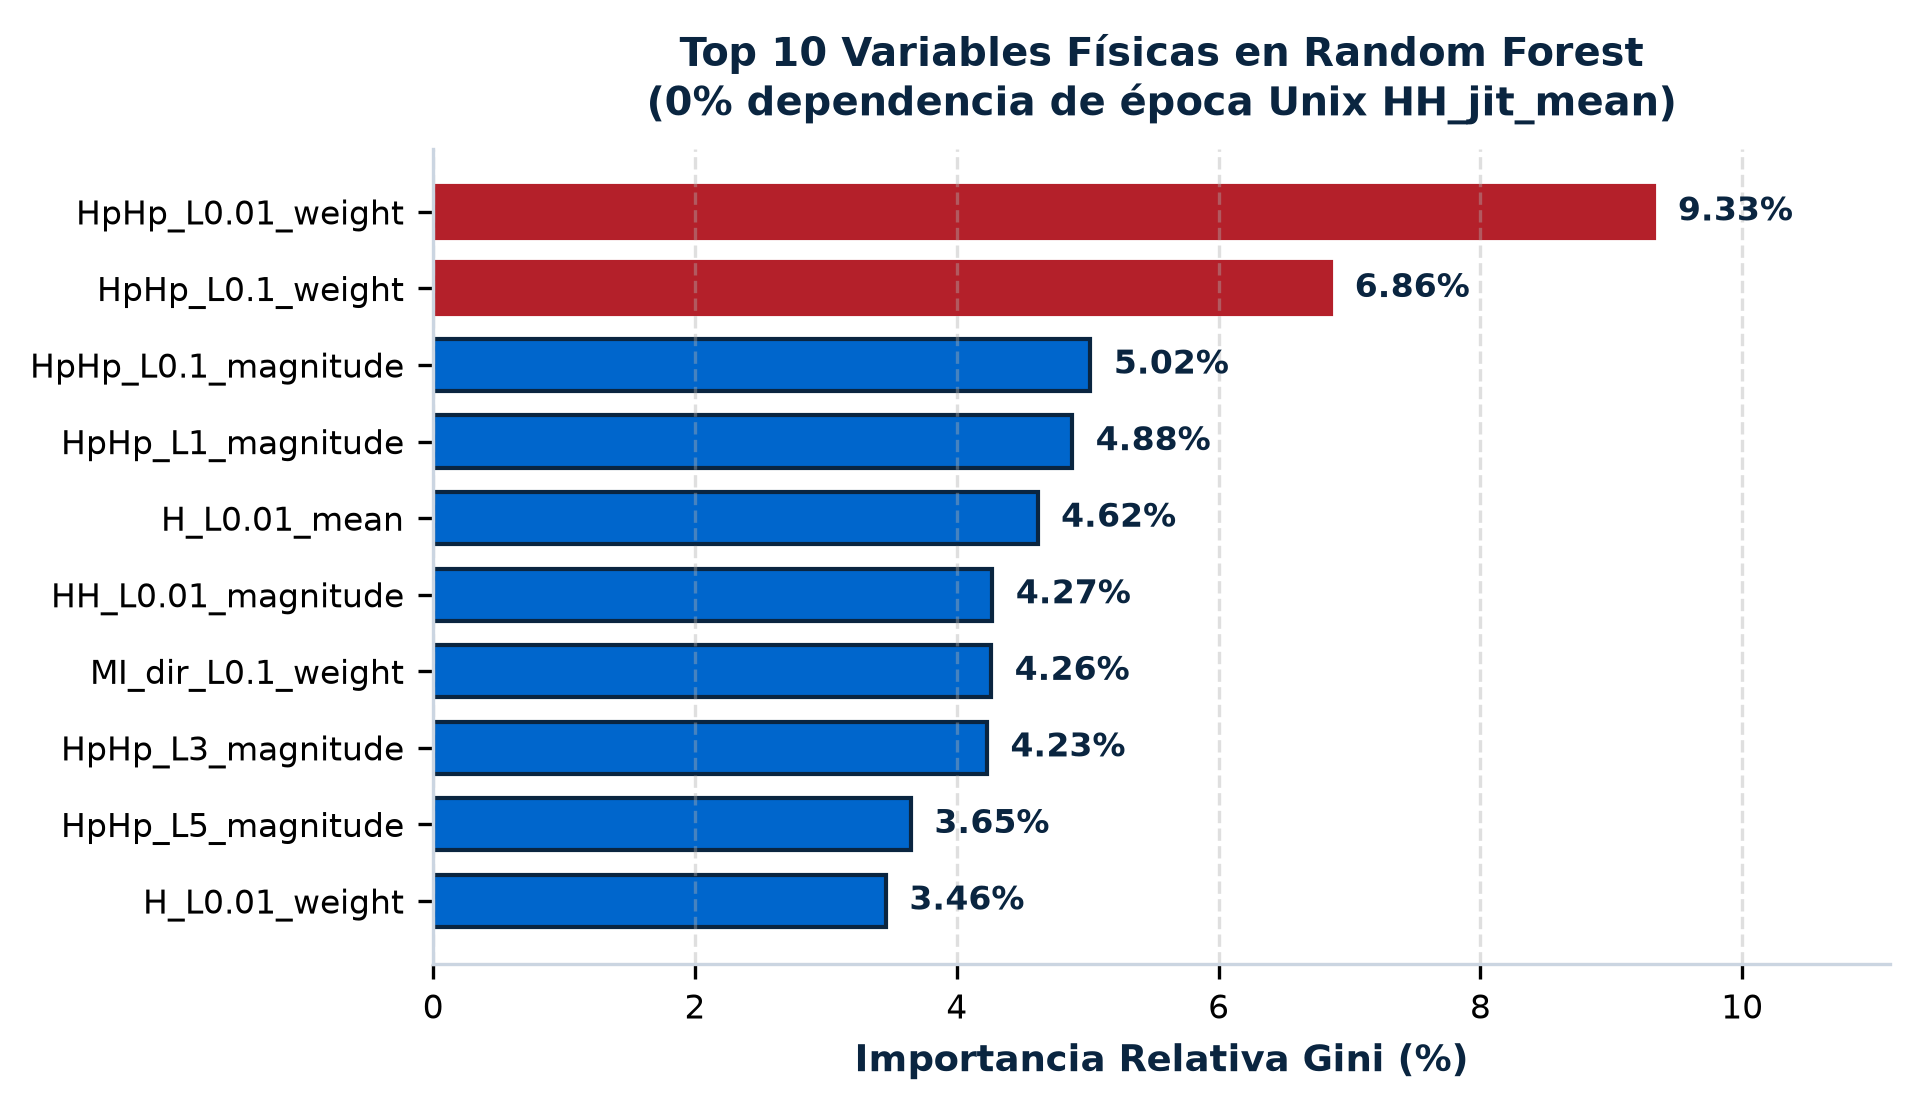
\includegraphics[width=0.98\linewidth,height=13.0cm,keepaspectratio]{fig_ppt_importancia_rf.png}\\[2mm]
  }{}
  {\fontsize{14}{18}\selectfont\color{CINFGray}\textbf{Figura 2.} Top 10 variables físicas en Random Forest tras el saneamiento (0\% dependencia del reloj Unix; Top 15 concentra 65,25\%).}
}

% -----------------------------------------------------------------------------
% FILAS 10-16 (ROWSPAN=7): FILA CENTRAL DE 3 COLUMNAS
% -----------------------------------------------------------------------------
\posterbox[
  colframe=CINFAccent, colbacktitle=CINFAccent,
  title={4. Arquitectura Doble Pipeline y Defensa en 3 Anillos}
]{name=box4, column=1, span=2, row=10, rowspan=7}{%
  Desacopla el entrenamiento (\textbf{Pipeline Offline}) de la clasificación en vivo (\textbf{Pipeline Online}) mediante artefactos verificados con \texttt{SHA-256}:
  \vspace{2mm}
  \begin{tcolorbox}[colback=CINFAccent!7, colframe=CINFAccent, boxrule=1.4pt, arc=3mm, left=4.5mm, right=4.5mm, top=3mm, bottom=3mm, no shadow]
    {\fontsize{16}{20}\selectfont\textbf{Anillo 1 — Detector Binario Ciego (Random Forest 6/2/1):} 9 modelos en rotación (\texttt{device\_1\_rf}--\texttt{device\_9\_rf}). Complejidad $O(k \cdot \text{prof.})$, \textbf{5,28 ms} CPU, 0,3--2,5 MB y umbral calibrado ($\text{FPR}\le 0{,}1\%$).}
  \end{tcolorbox}
  \vspace{1.5mm}
  \begin{tcolorbox}[colback=CINFBlue!7, colframe=CINFBlue, boxrule=1.4pt, arc=3mm, left=4.5mm, right=4.5mm, top=3mm, bottom=3mm, no shadow]
    {\fontsize{16}{20}\selectfont\textbf{Anillo 2 — Clasificador de Firma Botnet (Multiclase):} Identifica 10 subtipos de Mirai y BASHLITE sin etiquetas externas (\textbf{91,76\%} exactitud canónica; $F1_{\text{macro}} = 0{,}9173$).}
  \end{tcolorbox}
  \vspace{1.5mm}
  \begin{tcolorbox}[colback=CINFRed!7, colframe=CINFRed, boxrule=1.4pt, arc=3mm, left=4.5mm, right=4.5mm, top=3mm, bottom=3mm, no shadow]
    {\fontsize{16}{20}\selectfont\textbf{Anillo 3 — Detector Zero-Day (\texttt{LocalOutlierFactor}):} Entrenado \textbf{100\% con tráfico benigno}. Logra \textbf{75,60\% de recall} sin firmas previas ($F1 = 0{,}8369$).}
  \end{tcolorbox}
  \vfill
  \par\noindent\textbf{Comparativa Histórica, Complejidad y Latencia CPU:}
  \par\vspace{1.5mm}\noindent
  {\renewcommand{\arraystretch}{1.15}\fontsize{14}{18}\selectfont
  \begin{tabularx}{\linewidth}{@{}X c c c@{}}
    \toprule
    \textbf{Modelo (Ref.\ Hist.)} & \textbf{Inferencia} & \textbf{F1 Hist.} & \textbf{Latencia} \\
    \midrule
    \texttt{Dummy} (Control) & $O(1)$ & 0,0000 & 0,01 ms \\
    Regresión Logística & $O(d)$ & 0,9767 & 0,13 ms \\
    SVM Calibrada & $O(d)$ & 0,9803 & 1,39 ms \\
    Gradient Boosting & $O(k\cdot\text{prof.})$ & 1,0000 & 1,03 ms \\
    \textbf{Random Forest} & $\mathbf{O(k\cdot\text{prof.})}$ & \textbf{1,0000} & \textbf{5,28 ms} \\
    \bottomrule
  \end{tabularx}}
}

\posterbox[
  colframe=CINFGreen, colbacktitle=CINFGreen,
  title={5. Protocolo Riguroso 6/2/1 (9 Folds Ciegos)}
]{name=box5, column=3, span=2, row=10, rowspan=7}{%
  Se ejecutaron \textbf{73 experimentos} rotando 6 equipos en ajuste (bloques 10\%, 30\%), 2 en calibración (50\%, 65\%) y \textbf{1 dispositivo 100\% excluido} (80\%, 95\%):
  \vfill
  \centering
  \IfFileExists{fig_ppt_protocolo_621.png}{%
    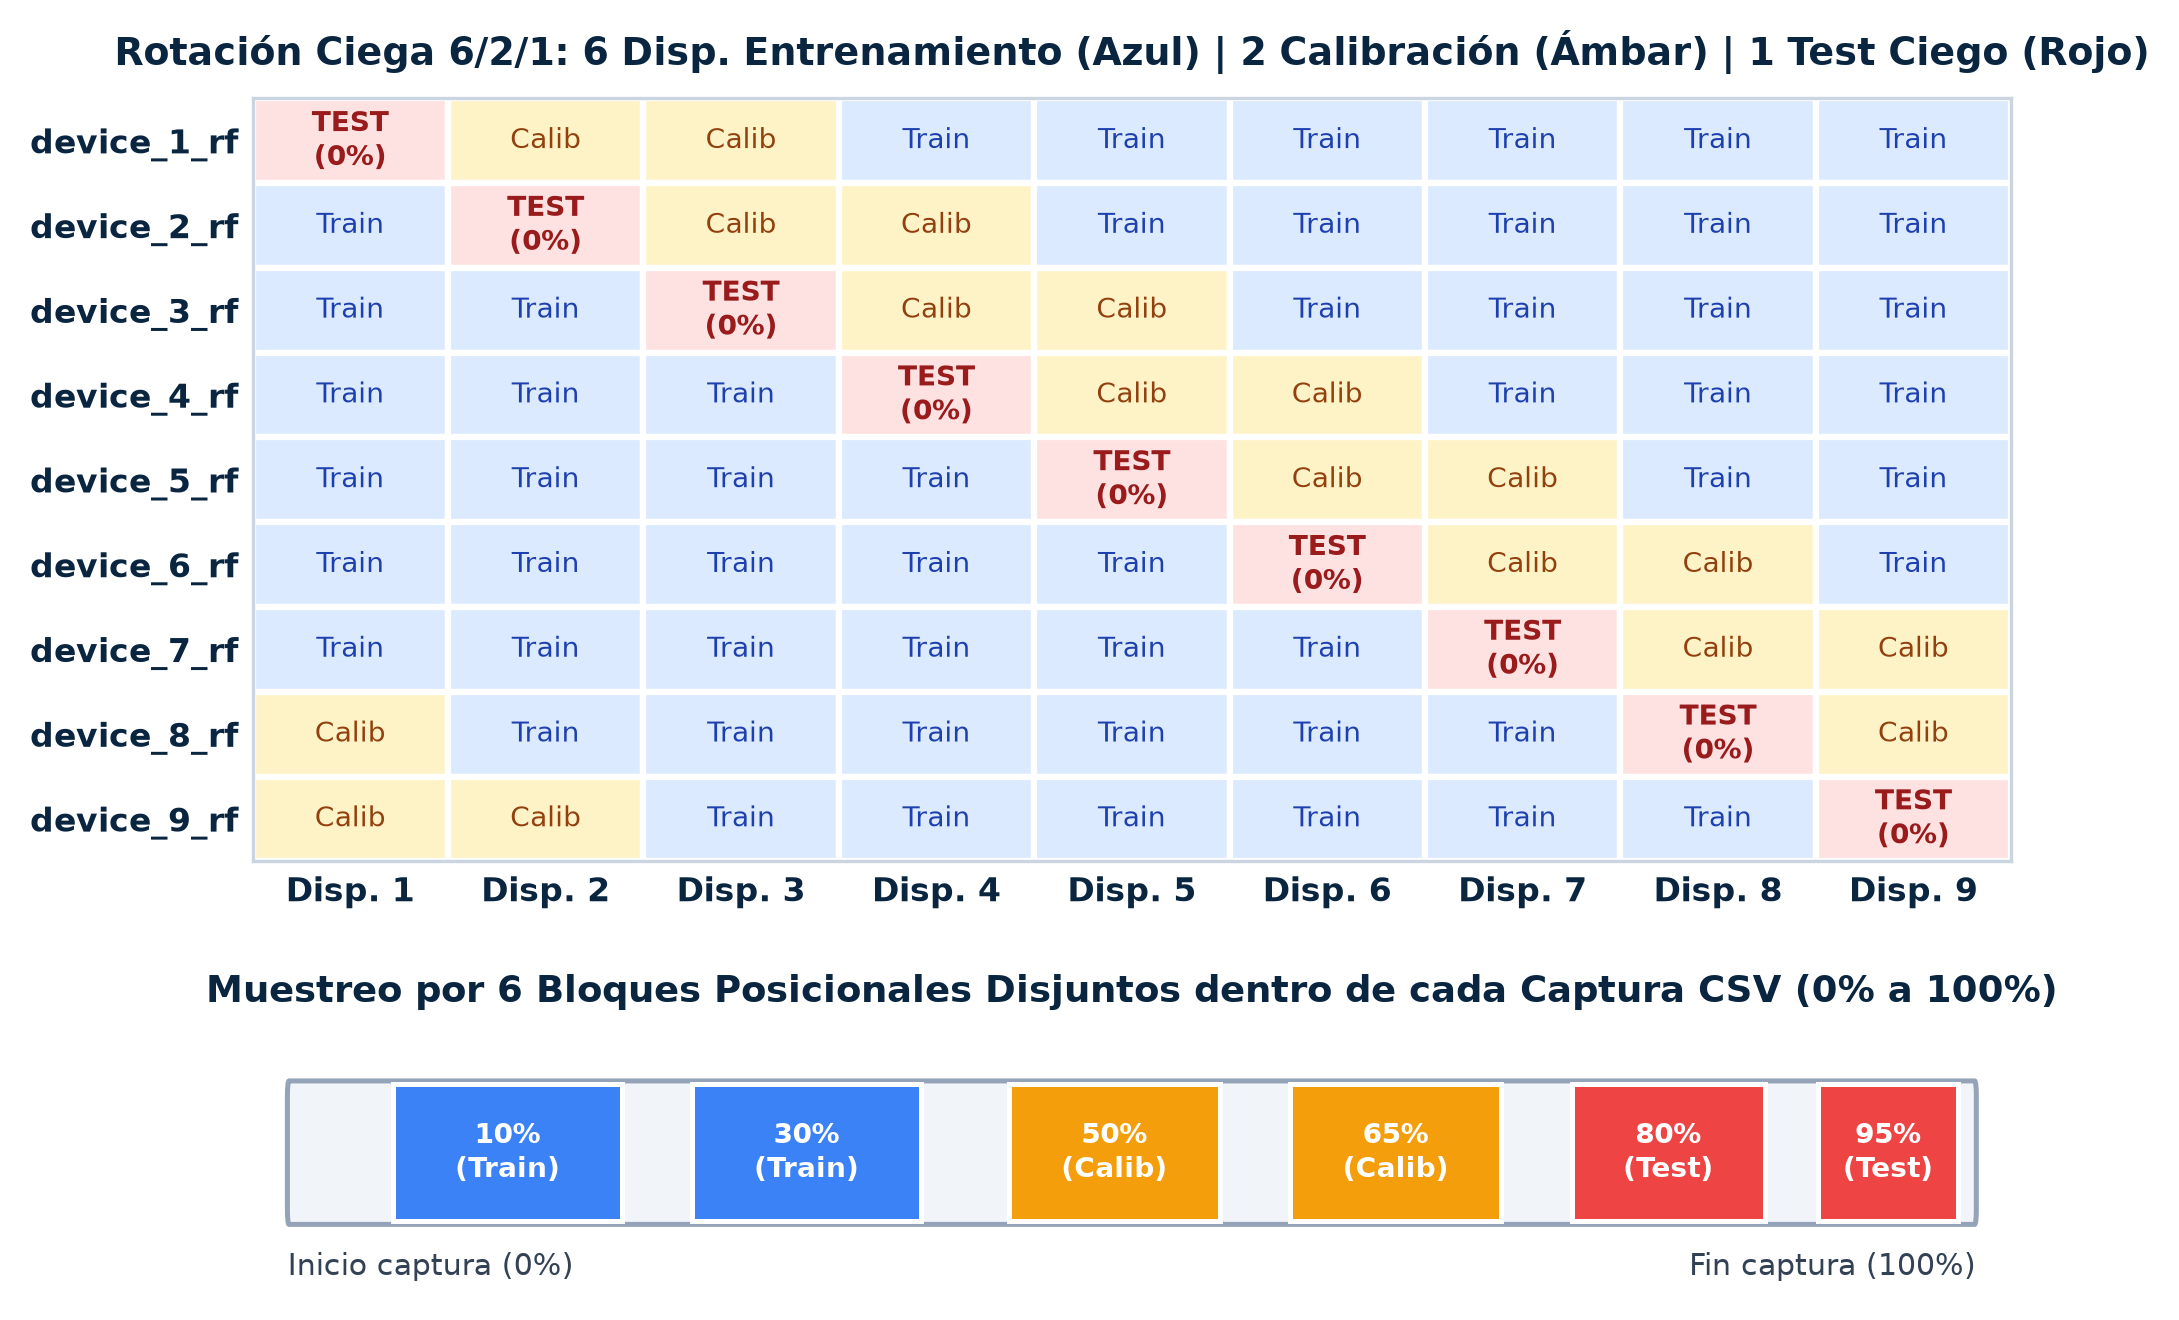
\includegraphics[width=0.99\linewidth,height=13.8cm,keepaspectratio]{fig_ppt_protocolo_621.png}\\[1.5mm]
  }{}
  {\fontsize{14}{18}\selectfont\color{CINFGray}\textbf{Figura 3.} Matriz de rotación ciega 6/2/1 y 6 bloques posicionales disjuntos.}
  \vfill
  \par\raggedright\noindent\textbf{Desempeño Externo por Dispositivo Excluido (9 Folds):}
  \par\vspace{1.5mm}\noindent
  {\renewcommand{\arraystretch}{1.15}\fontsize{14}{18}\selectfont
  \begin{tabularx}{\linewidth}{@{}X l c c c@{}}
    \toprule
    \textbf{Modelo} & \textbf{Umbral} & \textbf{F1 Med.} & \textbf{FPR} & \textbf{Min.\ Rec.} \\
    \midrule
    Reg.\ Logística & Fijo 0,5 & 0,9933 & 2,42\% & 99,45\% \\
    Reg.\ Logística & Ajustado & \textbf{0,8007} & 0,04\% & \textbf{22,62\%} \\
    Grad.\ Boosting & Ajustado & \textbf{0,9452} & 2,95\% & \textbf{60,00\%} \\
    \textbf{Random Forest} & Fijo 0,5 & \textbf{0,9998} & 0,05\% & 99,95\% \\
    \textbf{Random Forest} & \textbf{Ajustado} & \textbf{0,9995} & \textbf{0,14\%} & \textbf{99,95\%} \\
    \bottomrule
  \end{tabularx}}
}

\posterbox[
  colframe=CINFRed, colbacktitle=CINFRed,
  title={6. Prueba de Fuego Zero-Day y Ablaciones}
]{name=box6, column=5, span=2, row=10, rowspan=7}{%
  Al excluir una familia entera de botnet (16 escenarios) sobre hardware nunca visto, emerge el límite real del enfoque supervisado:
  \begin{itemize}
    \item \textbf{Sin Mirai (Disp.\ 4):} Recall cae a \textbf{39,90\%} ($F1=0{,}5702$; 1.202 ataques omitidos de 2.000).
    \item \textbf{Sin BASHLITE (Disp.\ 6):} Recall cae a \textbf{48,55\%} ($F1=0{,}6537$; 1.029 omisiones).
  \end{itemize}
  \vfill
  \centering
  \IfFileExists{fig_ppt_zeroday_caida.png}{%
    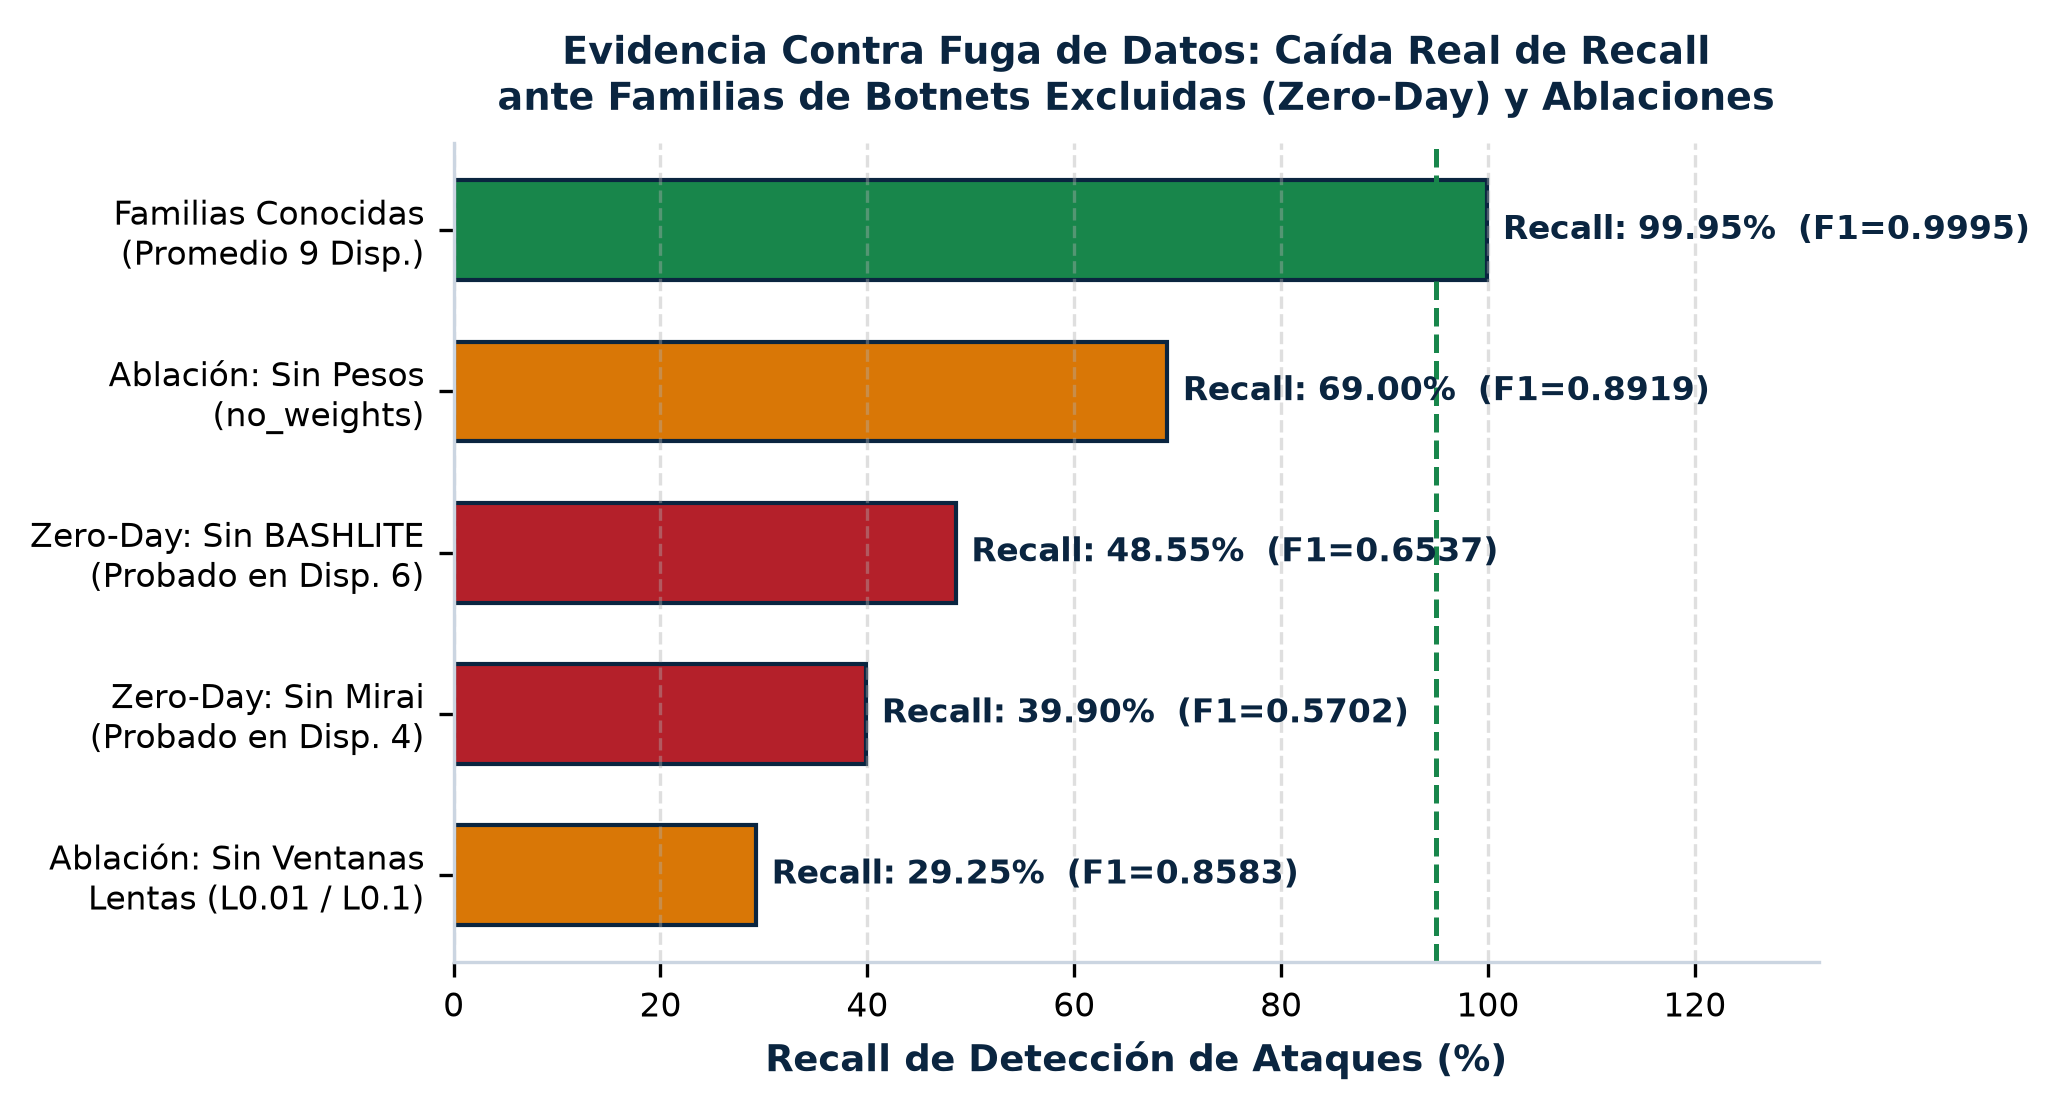
\includegraphics[width=0.98\linewidth,height=12.4cm,keepaspectratio]{fig_ppt_zeroday_caida.png}\\[1.5mm]
  }{}
  {\fontsize{14}{18}\selectfont\color{CINFGray}\textbf{Figura 4.} Contraste entre familias conocidas (99,95\%), ablaciones y caída real en Zero-Day.}
  \vfill
  \par\raggedright\noindent\textbf{Ablación de Características (Random Forest 6/2/1):}
  \par\vspace{1.5mm}\noindent
  {\renewcommand{\arraystretch}{1.15}\fontsize{14}{18}\selectfont
  \begin{tabularx}{\linewidth}{@{}X c c c@{}}
    \toprule
    \textbf{Representación} & \textbf{F1 Med.} & \textbf{FPR} & \textbf{Min.\ Rec.} \\
    \midrule
    \textbf{Sanitizada (105 vars.)} & \textbf{0,9995} & \textbf{0,14\%} & \textbf{99,95\%} \\
    Jitter crudo (con fuga) & 0,9988 & 0,30\% & 99,98\% \\
    Sin pesos (\texttt{weight}) & 0,8919 & 0,60\% & 69,00\% \\
    \textbf{Sin ventanas lentas} & \textbf{0,8583} & \textbf{0,56\%} & \textbf{29,25\%} \\
    \bottomrule
  \end{tabularx}}
}

% -----------------------------------------------------------------------------
% FILAS 17-23 (ROWSPAN=7): FILA INFERIOR DE 2 TARJETAS ANCHAS
% -----------------------------------------------------------------------------
\posterbox[
  colframe=CINFBlue, colbacktitle=CINFBlue,
  title={7. Consola Operativa MVP y Controles de Ciberseguridad}
]{name=box7, column=1, span=3, row=17, rowspan=7}{%
  \centering
  \IfFileExists{dashboard_funcionando.png}{%
    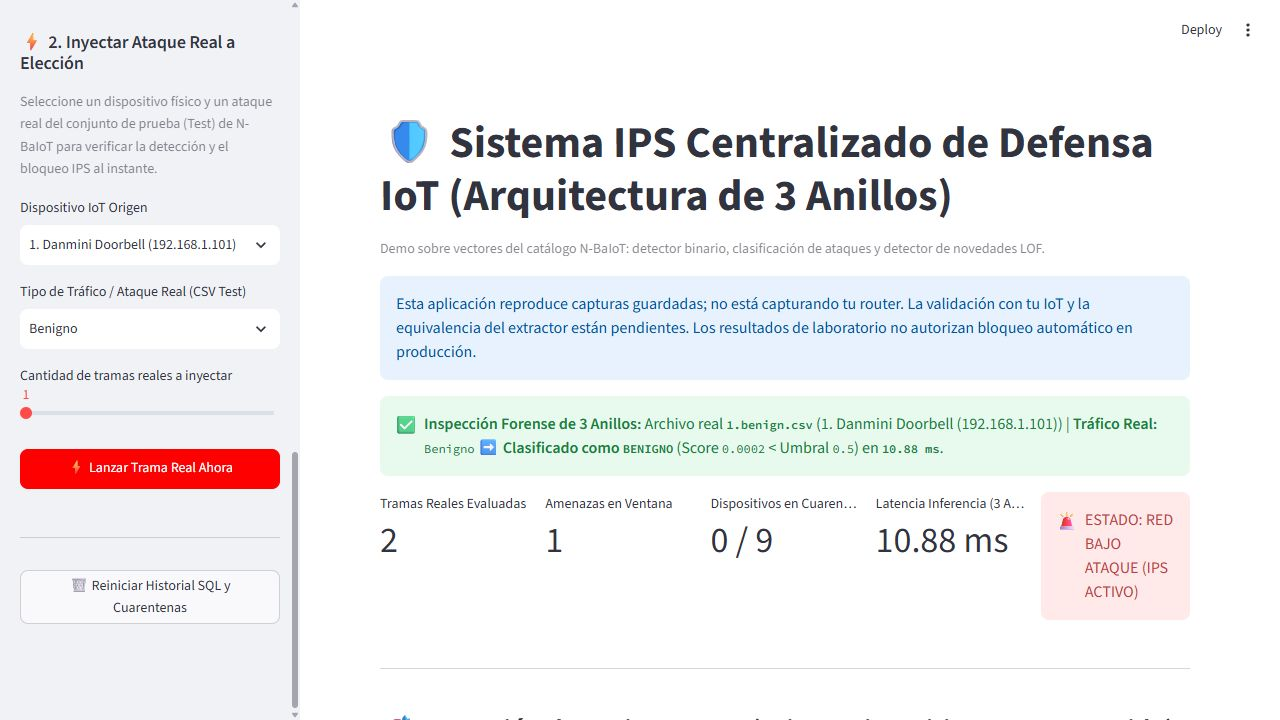
\includegraphics[width=0.96\linewidth,height=15.0cm,keepaspectratio]{dashboard_funcionando.png}\\[2mm]
  }{}
  {\fontsize{14.5}{18.5}\selectfont\color{CINFGray}\textbf{Figura 5.} Consola SOC en Streamlit (\texttt{localhost:8501}) ejecutando enrutamiento ciego 6/2/1, telemetría en vivo y causa raíz Z-Score.}
  \vfill
  \raggedright
  \begin{minipage}[t]{0.48\linewidth}
    \vspace{0pt}
    \begin{itemize}
      \item \textbf{Enrutamiento Ciego:} Inyectar tráfico en el Dispositivo $X$ activa \texttt{device\_X\_rf} (0\% visto en Train/Calib).
      \item \textbf{Control de Acceso:} Login \textbf{JWT \texttt{HS256}} con comparación en tiempo constante.
      \item \textbf{Integridad MLOps:} Verificación criptográfica \textbf{SHA-256} antes de cada \texttt{joblib.load()}.
    \end{itemize}
  \end{minipage}\hfill
  \begin{minipage}[t]{0.48\linewidth}
    \vspace{0pt}
    \begin{itemize}
      \item \textbf{Forense SQLite:} Consultas 100\% parametrizadas y rastreo del \textbf{Paciente Cero}.
      \item \textbf{Firewall Capa 2/3:} Reglas \texttt{iptables}/\texttt{nftables} (IP+MAC) con \textbf{Whitelist} (\texttt{192.168.1.1}).
      \item \textbf{Calidad y Onboarding:} \textbf{25/25 pruebas} ($0{,}86$~s) + Modo Aprendizaje 24h e Invitados.
    \end{itemize}
  \end{minipage}
}

\posterbox[
  colframe=CINFNavy, colbacktitle=CINFNavy,
  title={8. Discusión Crítica, Conclusiones y Proyección 2027}
]{name=box8, column=4, span=3, row=17, rowspan=7}{%
  \textbf{Discusión e Impacto:} A diferencia de métricas estáticas cercanas al 99,9\%, nuestros 73 experimentos confirman la fragilidad \textit{cross-domain} reportada por Wardana et al.\ (2024) y Bhilwarawala et al.\ (2026). La caída a \textbf{39,90\%} en Zero-Day constituye evidencia directa de \textbf{ausencia de fuga de datos} y valida la arquitectura híbrida de 3 anillos. El sistema promueve ciberseguridad local y privada sin inspeccionar \textit{payload} cifrado ni enviar tráfico a la nube.

  \vspace{2.5mm}
  \textbf{Limitaciones Declaradas:} Dataset capturado en 2018; bloques balanceados no miden FPR diario real; la consola opera sobre reproducción CSV quedando pendiente la validación numérica del extractor $O(1)$ en paquetes crudos.

  \vfill
  \par\noindent\textbf{Hoja de Ruta de Continuidad Experimental (2027):}
  \par\vspace{1.5mm}\noindent
  {\renewcommand{\arraystretch}{1.18}\fontsize{14.5}{18.5}\selectfont
  \begin{tabularx}{\linewidth}{@{}p{5.2cm} p{3.8cm} X@{}}
    \toprule
    \textbf{Etapa / Sprint} & \textbf{Periodo} & \textbf{Objetivo Técnico en Red Real} \\
    \midrule
    Etapa 8 (Sprint 4) & Mar--Abr 2027 & Despliegue \textit{Edge} en Raspberry Pi (benchmark ARM CPU/RAM). \\
    Etapa 9 (Sprint 5) & Abr--May 2027 & Certificación del extractor $O(1)$ sobre capturas \texttt{.pcap} en vivo. \\
    Etapa 10 (Sprint 6) & May--Jun 2027 & Medición de FPR real en hogar + políticas controladas OpenWrt. \\
    Etapa 11 (Sprint 7) & Jun--Jul 2027 & Autoencoder liviano cuantizado para elevar detección \textit{Zero-Day}. \\
    \bottomrule
  \end{tabularx}}

  \vfill
  \par\noindent\textbf{Referencias Clave:}\par\vspace{1mm}
  {\fontsize{13.5}{17.5}\selectfont\color{CINFGray}
  [1] Meidan et al. (2018), \textit{N-BaIoT: Deep Autoencoders}, IEEE Pervasive Computing. \quad
  [2] Chapman et al. (2000), \textit{CRISP-DM 1.0}. \quad
  [3] Studer et al. (2021), \textit{Towards CRISP-ML(Q)}, MAKE 3(2). \quad
  [4] Wardana et al. (2024), \textit{Ensemble Averaging DNN for Heterogeneous IoT}, Scientific Reports. \quad
  [5] Bhilwarawala et al. (2026), \textit{BRIDGE and TCH-Net Cross-Domain IoT Benchmark}, arXiv:2604.11324.
  }
}

% -----------------------------------------------------------------------------
% FILA 24: PIE DE PÁGINA PROFESIONAL
% -----------------------------------------------------------------------------
\posterbox[
  colback=CINFNavy,
  colframe=CINFNavy,
  valign=center,
  left=11mm, right=11mm, top=3mm, bottom=3mm
]{name=footer, column=1, span=6, row=24, rowspan=1}{%
  \begin{minipage}[c]{0.67\linewidth}
    {\color{white}\fontsize{18}{22}\selectfont\textbf{Reproducibilidad y Código Abierto:} \texttt{https://github.com/FelipeNVR/proyecto-iot-ml}}\\[1.5mm]
    {\color{white!78}\fontsize{15}{18}\selectfont Contacto: Felipe Nicolás Vergara Rodríguez (\texttt{f.vergararodrguez@uandresbello.edu}) · Universidad Andrés Bello, Viña del Mar}
  \end{minipage}\hfill
  \begin{minipage}[c]{0.30\linewidth}
    \raggedleft
    {\color{white!92}\fontsize{16}{20}\selectfont\textbf{Demo Interactiva en Vivo}}\\[1mm]
    {\color{white!75}\fontsize{14}{17}\selectfont Consola Streamlit · 9 Folds Ciegos 6/2/1 · 25 Tests OK}
  \end{minipage}%
}

\end{tcbposter}

\end{document}
